\chapter{Lotka-Volterra equations and considerations on the affect of each species}

In this chapter, we present a model for the evolution of the population between preys and predators. For predator and prey populations, we define a function that quantify the size of the population with respect to time. The goal is to motivate a choice of differential equations that will describe the interaction and give a possible evolution of the two populations. Lotka-Volterra equations are well known equation in mathematical biology. To get straight to the point, the equations are
$$\begin{cases}
\dot{x} = x(\a-\b y),\\  
\dot{y} = y(-\g + \d x).
\end{cases}$$
where $x$ and $y$ represent the size of the population of preys, and predators respectively. The parameters $\a,\b,\g,\d$ are positive scalars. In the first chapter we presented a pragmatic and mathematical analysis of the linear systems. Here, we propose first to speak about the qualitative understanding of the equation. We will progressively motivate the choice behind this modelisation by showing equations related to it, and then assert a modification on the equations that will give us more possible equations but for which the same study still works as in the classic system.

\section{Motivation} \label{sec:motiv}
We go back to the basics and remind that for a function $x$ of one variable $t$, the notations
\[x'(t) = \frac{\dd}{\dd t}x(t) = \dotx(t)= \lim_{h\to0}\frac{x(t+h)-x(t)}{h}\] 
are the derivative when the limit exist. Qualitatively it indicates the amount of change of the function with respect to the variable. This amount is absolute with respect to the size of $x$ and doesn't depend relatively on it. In consequence, when $x$ is non null which is an assumption we will always make for initial value, $\frac{\dot{x}}{x}$ quantify the relative rate of change of the function. This could be in our situation the mean number of descendant of an individual. For example if a specie reproduce itself always with the same speed no matter the population or the environment, we can say that their grow rate is a constant c:
\[ \dot{x} = cx, \]
If the population is positive, 
\[ \frac{\dot{x}}{x} = \frac{d}{dt}(\log{x}) = c \]
and then by integrating,
\[ \log{x(t)} = ct + \log{x(0)}, \]
giving us $x(t) = x(0)e^{ct}$, the exponential growth. This is quite intuitive, if a population double each step time the general formula is of powers of two, the population will just grow indefinitely. Alternatively if $c$ is taken negative, it mean we have loss of individuals, and the population decrease.
 
Obviously, this is doesn't encapsulate the reality as the function grow very fast forever. The growth rate must decrease as the population increase. This come from multiple complex reasons such as competition due to environment capacities in food, space etc. For now we suppose it is from the simplest form, a linear growth rate $\a -\b x$: 
\[ \dot{x} = x(\a -\b x) .\]
That gives us the logistic equation, where $\a$ represent the initial growth rate, and $\b$ how fast the growth rate slow down as the population size increase. Here we have one non trivial equilibrium when $\dot{x}(t)=0$ i.e. when $x(t)=\a/\b=x_*$. If not, we remark that $\dotx > 0$ when $ x < x_*$, and  $\dotx < 0$ when $ x < x_*$, meaning that $x_*$ seems stable. Indeed we do the computations and
\begin{IEEEeqnarray*}{rCl}
   \a = \dotx\frac{x_*}{x(x_*-x)}
   = \frac{\dotx}{x} + \frac{\dotx}{x_* - x}
   = (\log x + \log|x_* - x|)'.
\end{IEEEeqnarray*}
By integrating from 0 to t we get
\[ \a t  = \log(x(t)) - \log|x_* -x(t)| -( \log(x_0) - \log|x_* -x_0|)
= \log \frac{x(t)(x_* -x_0)}{x_0(x_*-x(t))} \]
and rearranging terms
\[x(t) = \frac{x_0x_*e^{\a t}}{x_* + x_0(e^{\a t}-1)} \]
which is well defined for $t\in\R$ if $0<x_0<x_*$, and for $t\in[1/\a \log(1 - x_*/x_0),\infty]$ if $0<x_*<x_0$. We see that in both cases $x(t)\to x_*$ as $t\to\infty$.
\begin{figure}[H]
    \centering
    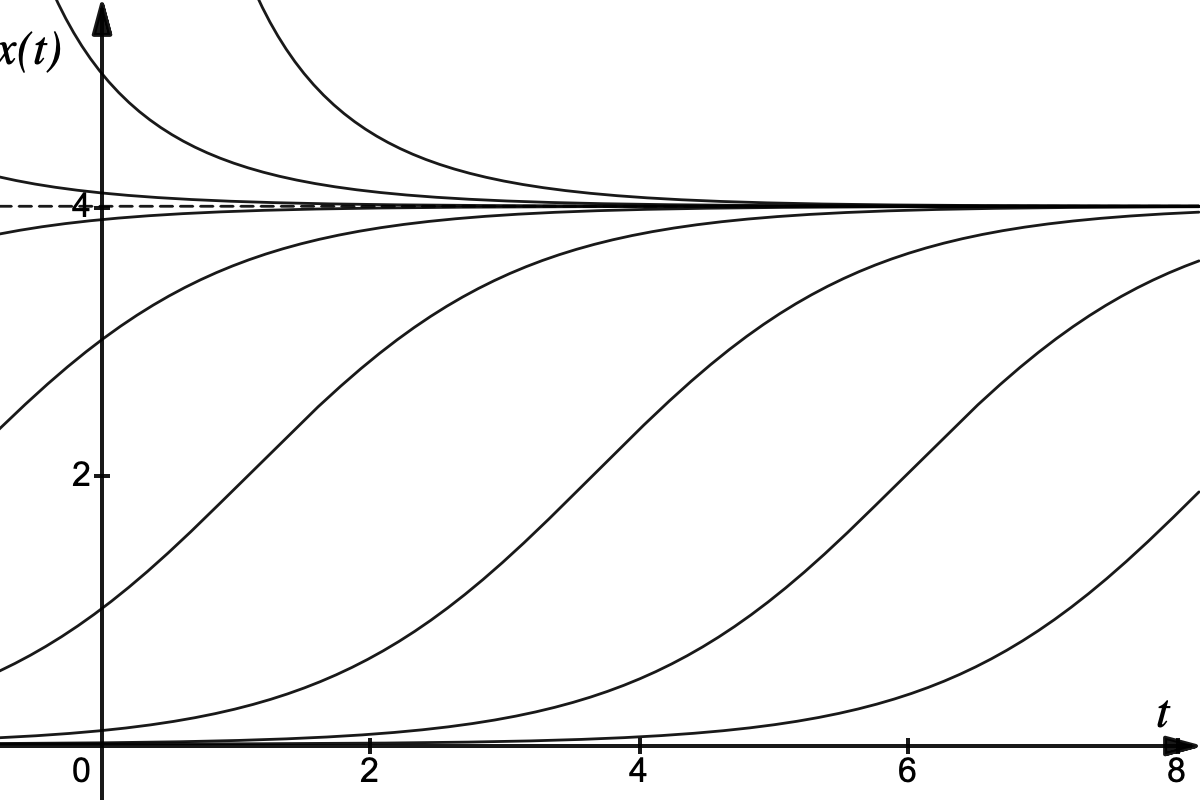
\includegraphics[scale=0.2]{images/logistic.png}
    \caption{Logistic equation for some initialisations, with $x_*=4$ and $\a=1$.}
    \label{fig:logistic}
\end{figure}

In conclusion for this logistic growth, the population will always stabilise in the direction of a unique non trivial equilibrium.

Now we want to introduce a second specie, the predator which alter the growth of the prey population, the same way we made the size of the population itself affect the rate of change. That mean that the growth rate will decrease in function of the prey, let's say linearly:
\[ \dotx = x(\a -\b y).\]
In the opposite, the growth rate of the predator increase together with the population. But it decrease without them:
\[ \doty = x(-\g +\d x).\]
This is the Lotka-Volterra equations for a prey-predator system.
When we added the affect of the other species, with didn't keep the affect of the population on itself. We can consider both of these affects and add a term in each growth rate:
  \begin{equation*}
    \begin{cases}
    \dotx &= x(\a -\b y - \m x) \\
    \doty &= y(-\g +\d x - \n y).
    \end{cases}
    \end{equation*}
We obtained the equations we wanted to investigate. Let us talk deeper about them and about the possible modifications:

The idea is that we want to be able to modify the way the size of the species affect the rate. Traditional Lotka-Volterra equation consider the rate of growth as linear with respect to the populations, let's change that. We use functions $F$ and $G$ that are strictly monotonic, hence bijective, and increase from $0$ to $\infty$ to replace the linearity:
\begin{equation} \label{eq:LV}
    \begin{cases}
    \dotB = F(B)(\a -\b G(\P)), \\
    \dotP = G(\P)(-\g +\d F(B)).
    \end{cases}
\end{equation}
Here again, $\a,\b,\g,\d$ are positive scalars.

Note that $F(B)$ and other similar forms are an abuse of notation and mean $F\circ B$. When using the dot notation we always mean derivation with respect to time. So if a function has not time as an argument, for example $F$, then
$\dot{F}(B) = (F\circ B)'$ and $\dot{F}(B(t))= (F\circ B)'(t)=\ddt(F(B(t)))$.

Let us consider a real case where these considerations are meaningful.
The paper \cite{Gav} proposes marine phages and bacteria. In this case bacteria doesn't seem to be limited by the environment and their size. We can suppose the affect of itself as negligible against the affect of the phages. With the modification, the effective and the physical size of the phage population are not the same. It seem that one of them quantify as the power p of the other. The reason behind this choice is that in the traditional Lotka-Volterra equations, we assume one predator meets one prey at a time. Here laboratory tests tend to say that the important meetings are when two (or maybe three) phages meet a bacteria.

This consideration make the power of $p=2$ appear on the value of the page population in the equation. Indeed we first wanted to wrote $\dotP=\P(-\g+\d B)$ meaning that the amount of change is the interactions between phages and bacteria, something like phages$\times$bacteria. But we need two phages, so something like phages$\times$phages$\times$bacteria which gives $\dotP=\P^2(-\g+\d B)$. A similar thinking motivate the writing of $\dotB=B(\a-\b \P^2)$. In other words, we can say that they are hunting  teams of $p$ phages. For the mathematical study, we will keep general functions F and G that we can change in function of these kind of considerations on the affect.

\section{Mathematical study}
We have a non trivial equilibrium where $\dotB=\dotP=0$:
\[ B_* = F^{-1}(\g/\d), \quad \P_* = G^{-1}(\a/\b)\]
Note that if one of the two populations is constant, then the other must be constant too and they must be in this total equilibrium. Let's rewrite \prettyref{eq:LV} using this notation:
\begin{equation} \label{eq:LV*}
    \begin{cases}
    \dotB = \b F(B)(G(\P_*) - G(\P)), \\
    \dotP = \d G(\P)(-F(B_*) + F(B)).
    \end{cases}
\end{equation}
Now we can study the sign of the derivatives $\dotB$ and $\dotP$ and draw a phase plane. The positive values $B_*$ and $\P_*$ divide the positive plane $\R_+^2$ in four regions as follow:
$$\begin{matrix}
\dotB<0 \text{ and } \dotP<0 
& \dotB<0 \text{ and } \dotP>0 \\
\dotB>0 \text{ and } \dotP<0 
& \dotB>0 \text{ and } \dotP>0 .
\end{matrix}$$
Trajectories seem to turn around the center of equilibrium but we cannot see if the solutions are converging to the fixed point, are cyclic, or even diverging. To test this, we compute the linearlized system in purpose to use the \prettyref{th:linearisation} and possibly obtain asymptotic stability. If not we will not be able to conclude for the moment, but this will give a hint to search more.
\begin{IEEEeqnarray*}{C}
D_{B,\P} \begin{pmatrix}
    F(B)(\a -\b G(\P))\\
    G(\P)(-\g +\d F(B) )
\end{pmatrix} \\
= \begin{pmatrix}
    F'(B)(\a -\b G(\P))
    & -F(B)\b G'(\P)
    \\
    G(\P)\d F'(B)
    & G'(\P)(-\g +\d F(B))
\end{pmatrix} .
\end{IEEEeqnarray*}
We evaluate in the equilibrium and obtain
$$ \begin{pmatrix}
     0 & -F(B_*)\b G'(\P_*)
    \\
    G(\P_*)\d F'(B_*)   & 0
\end{pmatrix}. $$
This matrix has obviously imaginary eigenvalues because the characteristic polynomial is just $$\l^2 + F(B_*)\b G'(\P_*)G(\P_*)\d F'(B_*)$$
and vanishes in $\pm i\sqrt{F(B_*)\b G'(\P_*)G(\P_*)\d F'(B_*)}$. This means that the linearized system is elliptic, and we cannot conclude with the theorem we have. However, this gives a hint, the solutions might be cyclic, just like in the linearized version.

For this we search a first integral by taking the cross product of \prettyref{eq:LV*} and dividing by $F(B)G(\P)$:
\begin{IEEEeqnarray*}{rCl} 
    0 &=& \big(\dotB \d G(\P)(-F(B_*) + F(B))
        - \dotP \b F(B)(G(\P_*) - G(\P)) \big) \frac{1}{F(B)G(\P)} 
        \IEEEyesnumber \label{eq:1integral} \\
    &=& \d(-\frac{\dotB}{F(B)}F(B_*) + \dotB)
    -  \b(\frac{\dotP}{G(\P)}G(\P_*) - \dotP) \\
    &=& \Big(\d (-P(B)F(B_*) + B) -\b(Q(\P) G(\P_*))-\P)\Big)'
\end{IEEEeqnarray*}
where $P$ and $Q$ are primitives of $1/F$ and $1/G$, and exist because $F$ and $G$ are continuous. This give us a conserved quantity 
\begin{IEEEeqnarray*}{rCl}
V(B,\P) &=& \d \big(-P(B)F(B_*) + B\big) 
-\b\big(Q(\P) G(\P_*)-\P\big) \\
&=& V(B(0),\P(0)) \\
&=:& V_0
\end{IEEEeqnarray*}
Now we know then that $(B,\P) \in V^{-1}(\{V_0\})$, a closed set as V is continuous. To understand the level set, we compute the gradient:
$$\nabla V(B,\P)
= \big(\d( -\frac{F(B_*)}{F(B)} + 1) , 
-\b(\frac{G(\P_*)}{G(\P)}-1)\big)^\top.$$
It never vanishes, except in the equilibrium and is continuous. As a result, the level set doesn't have interior otherwise the function would be constant and the gradient null. Since we have the local unicity of the solution, the level set is actually a closed line, \ie the solutions are in an closed orbit. The following graph shows the trajectory of some solutions, and the direction in each part of the first quadrant:
\begin{figure}[H]
    \centering
    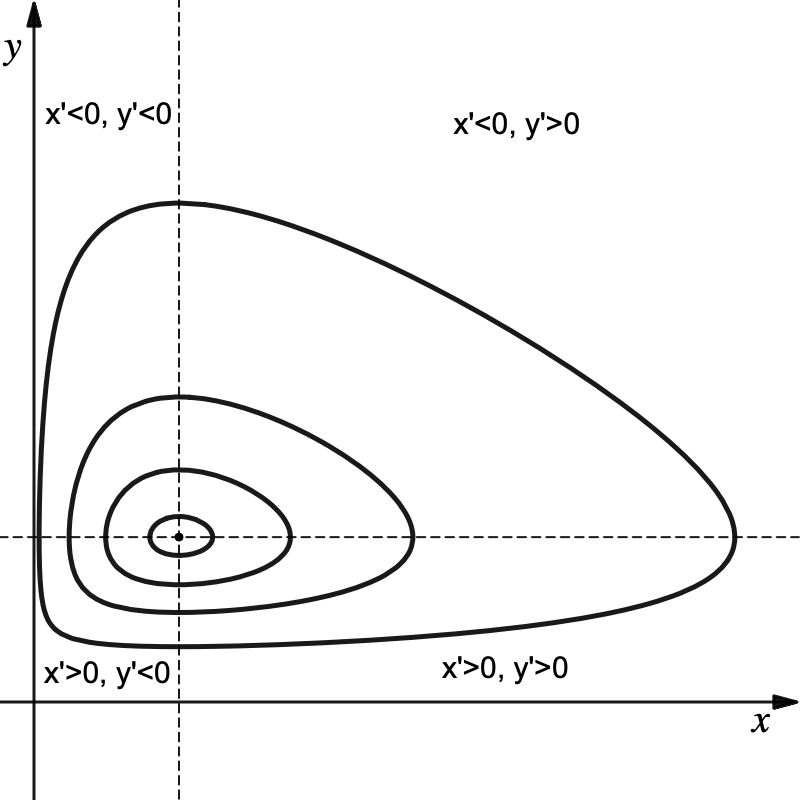
\includegraphics[scale=0.3]{images/LV.png}
    \caption{Some trajectories of the modified \LV system.\footnotemark}
    \label{fig:LV}
\end{figure}
\footnotetext{Interested readers can find \href{https://www.desmos.com/calculator/xsoo8fqwth}{here} an online interactive graphic that we made for the \LV system, and \href{https://www.desmos.com/calculator/go5ata2oee}{here} a version for the modified system. \\ (The urls are \emph{https://www.desmos.com/calculator/xsoo8fqwth} and \emph{https://www.desmos.com/calculator/go5ata2oee} .)}
Where we take $F=$Id, $G(\P)=\P^2$, and with a fixed point $(3.04,3.4)$. We see that as the formula of the gradient shows and the system itself, the extrema of $\P$ and $B$ are when the other function is on the equilibrium.
Now that we know that it's cyclic with a period $\tau$, we derive a modified Volterra principle by integrating these qualities obtained from \prettyref{eq:LV*}:
\[ \dotB / F(B) = \b (G(\P_*) - G(\P)). \]
the left side gives
\begin{IEEEeqnarray*}{rCl}
    \int_0^\tau \frac{\dotB}{F(B)} 
     &=& \int_0^\tau (P(B))'
     = P(B(\tau))-P(B(0)) =  P(B(0))-P(B(0)) =0,
\end{IEEEeqnarray*}
and then the rigth side
  \[ 0= \int_0^\tau \b (G(\P_*) - G(\P))
    = \tau\b G(\P_*) - \int_0^\tau \b  G(\P) \]
which implies that
 \[  G(\P_*) = \frac1\tau\int_0^\tau G(\P). \]
 Note that if $G=$Id, this says that the mean of the population $\P$ during time is $F(B_*)$. By the same argument with the second equation, we obtain that similarly
  \[  F(B_*) = \frac1\tau\int_0^\tau F(B). \]
  \\ \\
  In \prettyref{sec:motiv}, we explained how the own size of a population can affect its growth. We presented the logistic growth consequence of this equation:
  \[\dotx = x(\a - \b x).\]
  We add then a term in the rates of \prettyref{eq:LV} to modelise the fact that the growth rate of a population decrease with the size of population due to environment capabilities or competition. Again we use $F$ and $G$ to quantify their importance:
  \begin{equation} \label{eq:LV2}
    \begin{cases}
    \dotB &= F(B)(\a -\b G(\P) - \m F(B)), \\
    \dotP &= G(\P)(-\g +\d F(B) - \n G(\P)).
    \end{cases}
\end{equation}
with new positive scalars $\m$ and $\n$. We search for non trivial equilibrium where $\dotB_{**}=\dotP_{**}=0$ and obtain a linear system in $F(B_{**})$ and $G(\P_{**})$:
\begin{equation*}
    \begin{cases}
    -\a = - \m F(B_{**}) -\b G(\P_{**}), \\
    \g = \d F(B_{**}) - \n G(\P_{**}),
    \end{cases}
\end{equation*}
which give
\begin{IEEEeqnarray*}{rCl}
    \m\g-\d\a &=& \m\d F(B_{**}) - \m\n G(\P_{**}) - \d\m F(B_{**}) -\d\b G(\P_{**}) \\  &=& (-\m\n-\d\b) G(\P_{**}) 
\end{IEEEeqnarray*}
and then as $\m\n+\d\b > 0$ and supposing $\a\d>\g\m$
\begin{IEEEeqnarray}{rCl} \label{eq:Pstar}
G(\P_{**}) = \frac{\a\d-\g\m}{\b\d+\n\m} ,\quad
\P_{**}=P^{-1}\Big(\frac{\a\d-\g\m}{\b\d+\n\m}\Big).
\end{IEEEeqnarray}
Similarly,
\begin{IEEEeqnarray}{rCl} \label{eq:Bstar}
F(B_{**}) = \frac{\b\g+\n\a}{\b\d+\n\m}, \quad
B_{**} = F^{-1} \Big(\frac{\b\g+\n\a}{\b\d+\n\m}\Big).
\end{IEEEeqnarray}
Here we cannot derive a first integral like we did in \prettyref{eq:1integral} by separating variables $B$ and $\P$. Instead, we want to test the stability of $(\Bstar,\Pstar)$. First we can try to use the theorem of linearization to check the possible asymptotic stability of the system:
\begin{IEEEeqnarray*}{C}
D_{B,\P} \begin{pmatrix}
    F(B)(\a -\b G(\P) - \m F(B))\\
    G(\P)(-\g +\d F(B) - \n G(\P))
\end{pmatrix} \\
= \begin{pmatrix}
    F'(B)(\a -\b G(\P) - \m F(B)) - F(B)\m F'(B)
    & -F(B)\b G'(\P)
    \\
    G(\P)\d F'(B)
    & G'(\P)(-\g +\d F(B) - \n G(\P))-G(\P)\n G'(\P)
\end{pmatrix} .
\end{IEEEeqnarray*}
We evaluate in the equilibrium and obtain
$$ \begin{pmatrix}
     - F(\Bstar)\m F'(\Bstar) & -F(\Bstar)\b G'(\Pstar)
    \\
    G(\Pstar)\d F'(\Bstar)   & -G(\Pstar)\n G'(\Pstar)
\end{pmatrix}. $$

Now we could replace $F(\Bstar)$ and $G(\Pstar)$ by their expression \prettyref{eq:Bstar} and \prettyref{eq:Pstar}, and compute the characteristic polynomial. But we would still have the the expressions $F'(\Bstar)$ and $G'(\Pstar)$, that we know to be positive but nothing else. The polynomial isn't in a simple form and the computation of the eigenvalues become excessively cumbersome, because of the number of parameters and the hypothesis on them. More simply we show that a $2\times2$ matrix with the same signs of this one is always stable. Indeed all the factors are positives and we can write the matrix like
$$\begin{pmatrix}-a&-b\\c&-d\end{pmatrix}$$
with characteristic polynomial $\l^2+(a+d)\l+ad+bc$ of discriminant $(a+d)^2-4(ad+bc)$. If the discriminant is negative, then the real part of the root will be $-(a+d)/2<0$, and else $$\frac{-(a+d)\pm\sqrt{(a+d)^2-4(ad+bc)}}{2} 
< \frac{-(a+d) \pm (a+d) }{2} \leq 0$$
So the eigenvalues are stable and the linearized system too. By the theorem of linearization, the non-linear system is asymptotically stable in the equilibrium. In other words all solutions near enough this point tends to exponentially to it. However, we don't know how big is the basin of attraction.

\begin{comment}
 We propose here to fix things, we will check numerically for the example and see that even the numerical expression isn't simple. Let's say $F(B)=B$, $G(\P)=\P^2$ and fix arbitrary the parameters making attention to $\a\d>\g\m$. Let's say $\a=4$, $\b=5$, $\m=2$, $\g=1$, $\d=3$, $\n=6$.
We get then $\Bstar=F(\Bstar)
= (5\times1+6\times4)/(5\times3+6\times2)
= 29/27$, 
$F'(\Bstar)=1$, 
$\Pstar^2=G(\Pstar)
= (4\times3-1\times2)/(5\times3+6\times2)
= 10/27$, 
$G'(\Pstar)=2\Pstar=2\sqrt{10/27}$. The matrix is then
$$ \begin{pmatrix}
     - 29/27*2 & -29/27*5*2\sqrt{10/27}
    \\
    10/27*3   & -10/27*6*2\sqrt{10/27}
\end{pmatrix} 
= \begin{pmatrix}
    -58/27 & -290 \sqrt{10/3}/81 \\ 10/9 & -40\sqrt{10/3}/27
\end{pmatrix} 
$$
with the eigenvalues 
$$\l_1=\frac{1}{243} \big(-3 (87 + 20 \sqrt{30}) + 3 i \sqrt{3 (-6523 + 4060 \sqrt{30})}\big) 
\quad \text{ and } \quad \l_2=\bar{\l}_1.$$
We have then an stable linearized system
\end{comment}
For this we develop the theory of stability of Lyapunov. Consider a differential equation $\bdotx=\mathbf{F}(\mathbf{x})$, such that there exist a unique solution for each initial point and for all $t\geq0$. Such solutions are denoted by the flow $\phi$, such that $t\mapsto \phi(\mathbf{x}_0,t)$ is the solution initialised at $\mathbf{x}_0$. We recall the following definitions

\begin{definition}
 A fixed point $\mathbf{x}_*$ of  is said \emph{Lyapunov stable} or \emph{L-stable} if 
 for all $\epsilon>0$, there exists a $\delta>0$ such that for all $\mathbf{x_0}$ and for all $t\geq0$, $\|\mathbf{x_0} - \mathbf{x}_*\| < \delta$ implies $\|\phi(\mathbf{x_0},t) - \mathbf{x}_*\| < \epsilon$.
\end{definition}

\begin{definition}
A fixed point $\mathbf{x}_*$ of  is said \emph{attracting} if there exists a $\delta>0$ s.t. for all $\mathbf{x_0}$, $\|\mathbf{x_0} - \mathbf{x}_*\| < \delta$ implies that $\phi(\mathbf{x_0},t) \to \mathbf{x}_*$ as $t \to\infty$.
\end{definition}

\begin{definition}
    A fixed point which is L-stable and attracting is said \emph{asymptoticaly stable}
\end{definition}

\begin{remarque}
We remind that have shown that these two notions are different in \prettyref{rem:stabilité}.
\end{remarque}

Now we can introduce a tool that will be useful to understand the limit comportment of the trajectories and will a tool to proove asymptotic stability.

\begin{definition}
    Assume $\mathbf{x}_*$ is a fixed point of a equation $\bdotx = \mathbf{F}(\mathbf{x})$, and let a function $L:U\to\R$ defined in a neighbourhood of $\mathbf{x}_*$.
    \\
    The function $L$ is called a \emph{weak Lyapunov function} if \[L(\mathbf{x})>L(\mathbf{x}_*)\] 
    and 
    \[ \dot{L}(\xx):=\frac{\dd}{\dd t}L(\phi(\mathbf{x},t))|_{t=0} \leq 0 \]
    for all $\mathbf{x}$ in $U$.
    \\
    The function $L$ is called a \emph{Lyapunov function} (or a \emph{strict Lyapunov function}) provided that we have the strict inequality $\dot{L}(\xx) < 0$ when $\xx\neq\xx_*$.
\end{definition}

\begin{theoreme} \label{th:Lyapunov}
Let $\mathbf{x}_*$ a fixed point of the differential equation $\bdotx = \mathbf{F}(\mathbf{x})$ and $L$ a weak Lyapunov function on $U\ni\mathbf{x}_*$. Then $\mathbf{x}_*$ is L-stable. If $L$ is a strict Lyapunov function, $\mathbf{x}_*$ is attracting too and thus $L$ is asymptotically stable.
\end{theoreme}
\begin{proof}
L-stable: Let's suppose first that $L$ is a weak Lyapunov function. For any solution $\xx$, $\dot{L}(\xx) \leq 0$ and $L(\xx)$ is decreasing. Let be $\epsilon>0$. Up to taking it smaller, we suppose $B(\xx_*,\epsilon) \subset U$. But $L$ is continuous and $\partial B(\xx_*,\epsilon)$ is compact, we can then define
\[m=\min_{\partial B(\xx_*,\e)}{L} \; > \; L(\xx_*)=L_*,\]
and since $L$ is continuous, there exists a $\epsilon>\d>0$ such that $L_*<L(\xx)<m$ when $0<\|\xx-\xx_*\|<\d$. Now, for all solution starting in $ B(\xx_*,\d) \subset B(\xx_*,\epsilon)$, $L(\xx)<m$ mean that $\xx$ cannot go out of $B(\xx_*,\epsilon)$, otherwise it would cross $\partial B(\xx_*,\epsilon)$ in a certain $t>0$, and  we would have the contradiction $m>L(\xx(0)) \geq L(\xx(t))= m$. Whave the L-stability.

Attracting when strict Lyapunov: Since $L(\xx)$ is decreasing and bounded over $L(\xx_*)$, $L(\xx(t))$ must have a limit when $t\to\infty$, let's say $L_{\infty}$. This implies that $\dot{L}(\xx(t)) \to 0$. Using first part, let be $\d_2>0$ such that for all solution $\xx$ starting in $B(\xx_*,\d_2)$, and for all $t>0$, $\xx(t) \in B(\xx_*,\e)\subset U$. Now since $\xx(t)$ stay in a compact, there exists an accumulation point $\zz$ and a sequence $(t_n)_n$ growing to infinity such that $\lim_{n\to\infty} \xx(t_n) = \zz$. Because $\dot{L}$ is continuous, the limit $\lim_{n\to\infty} \dot{L}(\xx(t_n)) =0$ is actually $\dot{L}(\zz)=0$ and by hypothesis, $\zz$ must be $\xx_*$. Now because of the first part, as $\xx(t_n)$ approaches $\xx_*=\zz$, when $n$ is big enough $\xx(t_n)$ will be arbitrarily near from $\xx_*$ for all $t>t_n$, assuring the convergence for all $t\to\infty$, and $\xx_*$ is attracting.

From the two last parts we conclude that $\xx_*$ is asymptotically stable.
\end{proof}

We now return to our original problem: test the stability of $(\Bstar,\Pstar)$, the fixed point of
\begin{equation} \label{eq:LV3}
    \begin{cases}
    \dotB &= F(B)(\a -\b G(\P) - \m F(B)), \\
    \dotP &= G(\P)(-\g +\d F(B) - \n G(\P)).
    \end{cases}
\end{equation}
Generally speaking, there is no particular general method to find a Lyapunov function for generic equations. We note that concerning \prettyref{eq:LV}, we used a conserved quantity $V$ to prove periodicity of the trajectory. Let us try to use a similar version of this $V$ to obtain a quantity that would not be constant and for our goal, decreasing:
\[W(B,\P) = \d \big(-P(B)F(\Bstar) + B\big) 
-\b\big(Q(\P) G(\Pstar)-\P\big).\]
We compute its derivative along a solution $(B,\P)$:
\begin{IEEEeqnarray*}{rCl}
\dot{W}(B,\P) 
&=& \frac{\dd}{\dd t} \bigg(\d \big(-P(B)F(\Bstar)+B\big)
-\b\big(Q(\P) G(\Pstar)-\P\big)\bigg) \\
&=& \d \big(-\frac{\dotB}{F(B)}F(\Bstar) + \dotB\big) 
-\b\big(\frac{\dotP}{G(\P)} G(\Pstar)-\dotP\big) \\
&=& \d \frac{\dotB}{F(B)}\big(-F(\Bstar) + F(B)\big) 
-\b\frac{\dotP}{G(\P)}\big( G(\Pstar)-G(\P)\big) \\
&=& \d (\a -\b G(\P) - \m F(B))\Delta_F 
+\b(-\g +\d F(B) - \n G(\P))\Delta_G \\
&=& \d (\m F(B_{**}) +\b G(\P_{**}) -\b G(\P) - \m F(B))\Delta_F 
+\b(-\d F(B_{**}) + \n G(\P_{**}) +\d F(B) - \n G(\P))\Delta_G \\
&=& \d (-\m\Delta_F - \b\Delta_G)\Delta_F 
+\b(\d\Delta_F-\n\Delta_G)\Delta_G \\
&=& -\d\m\Delta^2_F - \b\n\Delta^2_G,
\end{IEEEeqnarray*}
with $\Delta_F= F(B)-F(\Bstar)$ and 
$\Delta_G= G(\P)-G(\Pstar)$. As a result, $\dot{W}(B,\P)$ is null only on $(\Bstar,\Pstar)$, otherwise it is strictly negative on $U=(\R^*_+)^2 \backslash\{(\Bstar,\Pstar)\}$. This is a Lyapunov function if we can prove that $(\Bstar,\Pstar)$ is a strict minimum. For this we simply compute the gradient and the Hessian:
$$\nabla W(B,\P)=(\d \big(-\frac{F(\Bstar)}{F(B)}+1\big) 
, -\b\big(\frac{G(\Pstar)}{G(\P)}-1\big))^\top$$
vanishes only in the fixed point, and
$$H_W(B,\P)=\text{diag}(\d\frac{F(\Bstar)F'(B)}{(F(B))^2} , \b\frac{G(\Pstar)G'(\P)}{(G(\P))^2})$$
is a diagonal matrix and has its eigenvalues in the diagonal. Because $F$ and $G$ are supposed positive and strictly increasing, the diagonal is strictly since its diagonal is strictly positive and we have supposed not being on the axes. As a result, the hessian is positive definite and $W$ is strictly convex, with a unique minimum on the only stationary point of $W$, the fixed point of the system. The function $W$ is Lyapunov and the fixed point is asymptotically stable.
For now, we don't know much about the size of the basin of attraction. Actually, in \prettyref{th:Lyapunov}, we have used the neighbourhood of the L-stability only because solutions would be bounded. We would like to prove a global convergence result. First we recall the notion: 
\begin{definition}
    A fixed point $\xx_*$ of $\bdotx=\mathbf{F}(\mathbf{x})$ is said \emph{globally attractive} on a set $U$, if for all $\mathbf{x_0}\in U$, $\phi(\mathbf{x_0},t) \to \mathbf{x}_*$ as $t \to\infty$. In other words it is attractive without condition on the proximity of the initial point.
\end{definition}
\begin{definition}
    A fixed point $\xx_*$ of $\bdotx=\mathbf{F}(\mathbf{x})$ is said \emph{globally asymptotically stable} on a set $U$, if it is globally attractive and L-stable. In other words it is asymptotically stable without condition on the proximity of the initial point for the convergence.
\end{definition}
Now, if we look at our proof of \prettyref{th:Lyapunov} on Lyapunov functions, we see that the proximity that we needed to obtain convergence, was just in purpose to have a compact and invariant set. Without loss of generality we can take the $\d_2$ as big as we want, as long as $\phi(B(\xx_*,\d_2)\times\R_+)$ is bounded in $U$. A criteria on the boundedness of $L^{-1}([L(\xx_*),L_0])$ will help us to obtain global attractivity:
\begin{corollaire}
Under the suppositions of \prettyref{th:Lyapunov}, if we have in addition that for a scalar $L_0>L(\xx_*)$,
\[ U_{L_0} = \{ \xx\in U | L(\xx) \leq L_0\} = L^{-1}\big([L(\xx_*);L_0]\big) \]
is bounded and whose closure is contained in $U$, then $\xx_*$ is globally asymptotically stable on $U_{L_0}$.
\end{corollaire}
\begin{proof}
First of all, $U_{L_0}$ is closed in the topology of $U$ because of the continuity of $L$. But since its euclidean closure is in U, it's actually closed in the all space. In addition, it is bounded, and thus, compact. Finally, all $\xx$ starting in $U_{L_0}$ will stay in $U_{L_0}$, because of the monotonicity of $L(\xx)$ and we have the convergence by the same argument of \prettyref{th:Lyapunov}, i.e. $L(\xx(t))\to L_\infty$, $\dot{L}(\xx(t))\to 0$, $\xx(t_n)\to \zz$ (because of the compacity of $U_{L_0}$), $\zz=\xx_*$, and $\xx(t)\to \xx_*$. This assure the global attractivity of $\xx_*$ on $U_{L_0}$, and hence, the global asymptotic stability, since the L-stability was assured yet.
\end{proof}

\begin{remarque}
If the hypothesis is true for all $L_0>L(\xx_*)$ then it is actually globally asymptotically stable everywhere on U. More generally, if a closed set $U_0\subset U$ (possibly $U$ itself), is invariant and each trajectory is bounded, we have global asymptotic stability on it.
\end{remarque}
We go back to our problem and recall that our Lyapunov function is 
\[W(B,\P) = \d \big(-P(B)F(\Bstar) + B\big) 
-\b\big(Q(\P) G(\Pstar)-\P\big)\]
defined in $(\R^*_+)^2$. For all $W_0>W(\Bstar,\Pstar)$, under the condition that $W$ tends to infinity when $B$ or $\P$ tends to infinity, $U_{W_0}=W^{-1}([W(B_*,\P_*);W_0])$ must be bounded and closed in the interior of the positive quadrant. If not, we would have a sequence inside $U_{W_0}$ converging to infinity or to the axes whose image by $W$ is bounded which is impossible by supposition. If $F=G=$Id for instance, it is obviously the case because $P=G=$log which explode in zero and is dominated by Id at infinity. In all cases, the convexity of $W$ and the strict min in the fixed point assures that at infinity the function indeed explodes. For the axes, we see that the form of $P(B)$ (similar for $Q(\P)$) can be written
$$P(B) 
= \int_{1}^B\frac{1}{F(B)}+c$$
and as $F(B)>F(0)=0$, it explodes to $-\infty$ if $F(B)$ become small enough when $B$ tends to zero. A sufficient condition for $F(B)$ is to be $O(B)$ for example. Then looking at the formula of $W$, it explodes to infinity too. The fixed point is globally asymptotically stable on the positive quadrant if $F$ and $G$ are $O(x)$ in zero.